% Informe de actividades profesionales
% Sergio Cuellar
% 26 Marzo 2011



% Define tamanio de papel y tamaño de la fuente, así como la clase book
\documentclass[12pt,oneside]{book}

% Permite usar acentos y ñ
\usepackage[utf8x]{inputenc}

% Define algunos paquetes a usar a lo largo del documento
\usepackage{amsmath}

\usepackage{amssymb}

\usepackage{latexsym}

% Convierte los títulos a español (Indice General, Capítulo, etc.)
\usepackage[activeacute,spanish]{babel}

% Para incluir imágenes
%\usepackage[pdftex]{graphicx}
\usepackage[dvips]{graphicx}

% Para que los headers se vean bonitos
\usepackage{fancyhdr}

% Para modificar margenes
\usepackage[letterpaper,top=3cm,bottom=2cm]{geometry}

% Para usar pstricks
\usepackage{pstricks}

% Para incluir urls
\usepackage{url}


% Para hacer referencias a etiquetas de otros documentos
\makeindex

% Esto ya no me acuerdo para que es
%\DeclareGraphicsRule{.gif}{eps}{.gif.bb}{`convert #1 'eps:-' }
%\DeclareGraphicsRule{.jpg}{eps}{.jpg.bb}{`convert #1 'eps:-' }

% Ruta para indicar en donde estan las imagenes a incluir
\graphicspath{{./images/}}

% Esto permite tener subsubsecciones
\setcounter{tocdepth}{99}
\setcounter{secnumdepth}{99}

% Para cuando se pongan tablas no diga Cuadro sino Tabla
% Cuadro se oye raro, aunque según los españoletes es lo correcto
% coño joder, jilipollas
\addto\captionsspanish{
\def\tablename{Tabla}
}

\begin{document}
\frontmatter
\tableofcontents

% Esto sirve para que entre parrafo y parrafo se deje un
% espacio en blanco definido por el primer número (los demás no sé
% qué signifiquen), ya que la clase book no lo tiene.
\setlength{\parskip}{3ex plus 0.5ex minus 0.2ex}

\mainmatter

% Objetivos
% Sergio Cuellar
% 26 Marzo 2011

\chapter{Objetivo}

\label{chap:objetivo}

Desarrollo e implementación de reportes que ayuden a la operación de restaurantes a eficientar sus procesos, conocer resultados, ahorrar tiempo, identificar áreas de oportunidad. Así como también el desarrollo de aplicaciones que ayuden a la mejora en el sistema en general del punto de venta utilizado.

La plataforma a utilizar es GNU/Linux utilizando Apache Tomcat, Java, JSP, Perl, C, Bash, y otras herramientas de software libre.
% Introduccion
% Sergio Cuellar
% 26 Marzo 2011

%Para que no tenga número en el indice un *
\chapter*{Introducción}
%pero para que sea añadido al indice
\addcontentsline{toc}{chapter}{Introducción}
\label{chap:intro}

La tecnología de la información (TI) es una herramienta valiosa dentro de la estrategia de negocios de Premium Restaurants Brand (PRB). En el departamento de Sistemas proveemos de soluciones tecnológicas a nuestros restaurantes, así como también establecemos estándares tecnológicos y de procesos en nuestras oficinas.

PRB maneja las marcas KFC y Pizza Hut, contando con más de 300 restaurantes a nivel nacional. El sistema operativo que se maneja en los restaurantes es GNU/Linux, teniendo como punto de venta (POS\footnote{Point of Sale}), un desarrollo propietario realizado en su origen por Yum Restaurant Brands de Estados Unidos.

Las Tecnologías de la Información apropiadas, cuando se utilizan junto con los principios de administración de ingresos, puede ayudar a los restaurantes a aumentar éstos y sus ganancias. Las Tecnologías de la Información han revolucionado el panorama de los negocios en el mundo y la industria de los restaurantes no es la excepción. Las TI han modificado a varias industrias y ahora juegan un papel fundamental en las reglas que rigen el mundo de los negocios y en la forma en que se acercan a los clientes. Las ventajas de las TI en cuanto al incremento de la competitividad, reducción de errores y creación de nuevas funcionalidades son incuestionables en cualquier sector, incluido el de los restaurantes.

Los restaurantes han invertido en automatización de funciones relacionadas con la nómina, contabilidad, inventario, etc., con el objetivo de bajar costos. También existen los sistemas punto de venta (POS, Point of Sale), los cuales facilitan sustancialmente la operación del restaurante, ayudando a realizar el marcaje de productos de manera rápida, con lo que se logra atender un mayor número de clientes en menor tiempo, la modificación automatizada de los menús, cambio de precios, etc.

En PRB contamos con un POS creado a la medida, lo cual permite a la empresa realizar desarrollos que implican la modificación del mismo POS, ya que se cuenta con el código fuente de éste. Estas modificaciones implican programación de nuevas funcionalidades o de corrección de errores (bugs). Así mismo es posible realizar desarrollos que se relacionen con el POS e interactúen con él, para la obtención y manipulación de datos generados por el punto de venta.

Diversas áreas de la empresa, como Operaciones y Finanzas, principalmente, considera los datos de la venta como muy importantes, ya que gracias a ellos pueden saber la tendencia que siguen las ventas, el comportamiento de los nuevos productos y/o promociones, los niveles de inventarios, los días y horas de mayores ventas, etc. 

Una de las actividades del área de Desarrollo de la Dirección de Sistemas, se encarga de la programación de reportes web de los datos que ayuden principalmente a los gerentes de restaurante a visualizar los datos de las operaciones de su restaurante de manera casi inmediata.

\section*{Objetivos}
\addcontentsline{toc}{section}{Objetivos}
\label{sec:objetivosss}

Desarrollo e implementación de reportes que ayuden a la operación de restaurantes a eficientar sus procesos, conocer resultados, ahorrar tiempo, identificar áreas de oportunidad. Así como también el desarrollo de aplicaciones que ayuden a la mejora en el sistema en general del punto de venta utilizado y de la operación del restaurante.

La plataforma a utilizar es GNU/Linux utilizando Apache Tomcat, Java, JSP, Perl, C, Bash, y otras herramientas de software libre.
% Perfil
% Sergio Cuellar
% 14 de mayo 2011

\chapter{Perfil}
\label{chap:perfil}

\textbf{Puesto Actual:} Programador Analista

\textbf{Puesto del Supervisor:} Gerente de Desarrollo de Restaurantes 

\textbf{Nombre del Supervisor:} Aníbal Avelar

\textbf{Propósito de la función:} Atender requerimientos relacionados al desarrollo de sistemas en restaurantes por parte del área de Operaciones y Sistemas.

%\textbf{Funciones de la posición:}

\section{Funciones de la posición}
\label{sec:func_posicion}


\begin{itemize}
 \item Desarrollo de reportes en restaurantes requeridos principalmente por el área de Operaciones.
 \item Desarrollo de scripts y programas que mejoren la operación del sistema del restaurante.
 \item Corrección y mejoras del sistema de punto de venta (SUS/FMS).
 \item Desarrollo de nuevas herramientas que coadyuven a la disminución del costo de operación.
\end{itemize}

%\textbf{Impacto de la Posición:}
\section{Impacto de la Posición}
\label{sec:empacto_posicion}


\begin{itemize}
 \item \textbf{Requerimientos técnicos:} GNU/Linux, Java, Perl, bash scripting, C/C++.
 \item \textbf{Conocimientos adquiridos en el puesto:} Funcionamiento de la operación del negocio. Así como también, el uso de otras tecnlogías nuevas que puedan ayudar al desarrollo de los sistemas.
 \item \textbf{Toma de decisiones:} El diseño y desarrollo de los reportes solicitados.
\end{itemize}

%\textbf{Relaciones de Trabajo:}
\section{Relaciones de Trabajo}
\label{sec:rel_trabajo}


\begin{itemize}
 \item \textbf{Internos:} Con el área de soporte técnico para la resolución de problemas escalados. Con el área de operaciones para obtener los requerimientos en reportes a desarrollar.
 \item \textbf{Externos:} Con franquicias para proporcionar soporte técnico y consultoría técnica en los reportes del sistema.
\end{itemize}

%\textbf{Perfil:}
\section{Características del perfil}
\label{sec:pperfil}


\begin{itemize}
 \item \textbf{Estudios:} Ing. en computación, ciencias de la computación y/o licenciatura en informática.
 \item \textbf{Experiencia mínima requerida:} 3 años
 \item \textbf{Habilidades requeridas:} Conocimientos en programación, en sistemas tipo UNIX, trabajo en equipo, conocimiento del idioma inglés, trabajo en equipo.
 \end{itemize}
% Desarrollo
% Sergio Cuellar
% 30 de abril 2011

\chapter{Desarrollo}
\label{chap:desarrollo}

El área de Desarrollo de Sistemas de Restaurantes está conformado por cuatro personas encargadas de proveer varios servicios de apoyo a alrededor de 340 restaurantes propios de la franquicia de PRB, así como alrededor de 150 restaurantes de otros franquiciatarios. Los requerimientos de desarrollos nuevos son proporcionados generalmente por el área de Operaciones cuando éstos tienen que ver la operación misma del restaurante, o bien, por la misma área cuando se deben realizar actualizaciones, corrección de bugs, etc., al sistema.

\section{Objetivos}
\label{sec:objetivos}

Entre los servicios proporcionados por el área de Desarrollo de Sistemas de Restaurantes se encuentran:

\begin{itemize}
 \item Desarrollo y mantenimiento de reportes solicitados por el área de Operaciones.
 \item Mantenimiento al punto de venta (programación de mejoras, nuevas funcionalidades, corrección de bugs).
 \item Programación de herramientas que coadyuven a la eficaz operación del restaurante.
 \item Desarrollo de aplicaciones que contribuyan a disminuir el costo de operación.
 \item Investigación de nueva infraestructura de sistemas en el restaurante (impresoras, tarjetas de vídeo, terminales, etc.)
\end{itemize}

\section{Descripción del Sistema en restaurantes}
\label{sec:descripcion}

Cada uno de los restaurantes cuenta con una computadora, en la cual se efectúan diversos procesos como son:

\begin{itemize}
 \item Registro y procesamiento de la venta.
 \item Generación de reportes.
 \item Manejo de periféricos como impresora de tickets, impresora del gerente, cajas registradoras, terminales, etc.
 \item Actividades gerenciales (correo electrónico, consultas web de la intranet, uso de procesador de textos, hoja de cálculo, etc).
\end{itemize}

\subsection{Software Libre}
\label{subsec:software_libre}

Una de las características principales del sistema en restaurantes, es que casi en su totalidad, a excepción del punto de venta que fue desarrollado por la compañía, es software libre.

El software libre es software que puede ser usado, estudiado y modificado sin restricción y el cual puede ser copiado y redistribuido en su forma modificada u original, ya sea sin restricciones o con mínimas restricciones que aseguren que los siguientes usuarios del software puedan seguir haciendo estas actividades. El software libre es generalmente disponible sin cargo alguno pero puede tener algunas cuotas, por ejemplo para ser distribuido en forma de CDs u otras formas.

En la práctica, para que un software sea distribuido como software libre, el código fuente de éste debe estar disponible para el usuario, así como también indicarle en una nota que se le conceden los derechos arriba mencionados. Esta nota puede ser, ya sea, una licencia de software libre o indicando que el código fuente está disponible al dominio público.

Las ventajas del software libre son:

\begin{itemize}
 \item Bajo costo, lo que implica el ahorro en pago de licencias.
 \item Es posible adaptar el software a las necesidades que tenga cada usuario, teniendo como resultado un software personalizado.
 \item Al ser público el código fuente, permite que programadores hagan correcciones a errores y mejoren el software de manera rápida.
 \item De acuerdo a los dos últimos puntos, el software libre no depende de una única empresa u organización, lo que evita que se impongan condiciones en su uso, como ocurre con el software privado.
 \item La innovación tecnológica que surge gracias a que cada usuario puede hacer aportaciones a la mejora del software.
\end{itemize}

El sistema de software de los restaurantes se compone principalmente de:

\begin{itemize}
 \item Sistema Operativo GNU/Linux kernel 2.6, basado en Knoppix con escritorio Xfce.
 \item Apache Tomcat
 \item Servidor HTTP Apache
 \item PostgreSQL
 \item Mozilla Firefox
 \item Mozilla Thunderbird
 \item OpenOffice.org
 \item Herramientas GNU (bash, ksh, awk, perl, etc.)
 \item Sistema punto de venta SUS/FMS (propietario, desarrollado por la misma compañía.
\end{itemize}

\subsection{GNU/Linux}
\label{sec:linux}

GNU/Linux se refiere al sistema operativo que utiliza el kernel Linux y las herramientas GNU. El kernel Linux puede ser instalado en una gran variedad de hardware, desde teléfonos móviles, computadoras tipo tableta, consolas de videojuegos, hasta mainframes y supercomputadoras. El kernel de Linux fue iniciado en 1991 por el finlandés Linus Torvalds. Las herramientas del sistema y librerías conocidas como GNU, fueron en un principio desarrolladas por Richard Stallman en 1983.

Algunas características del kernel de Linux son:

\begin{itemize}
 \item Es multitareas, permite ejecutar diferentes programas al mismo tiempo.
 \item Es multiusuario, distintos usuarios pueden estar conectados a la misma computadora al mismo tiempo.
 \item Es multiplataforma, puede ser instalado en distintos tipo de arquitectura de procesadores.
 \item Es multihilo, Linux tiene soporte en kernel nativo para el control de múltiples hilos independientes.
 \item Tiene soporte a una gran cantidad de sistemas de archivos (ext2, ext3, ext4, ReiserFS, XFS, JFS, FAT32, etc.).
\end{itemize}


\subsection{Apache Tomcat}
\label{sec:tomcat}

Apache Tomcat o simplemente Tomcat es un contenedor de servlets desarrollado por la Apache Software Foundation. Tomcat implementa las especificaciones de Java Servlet y JavaServer Pages (JSP) de Sun Microsystems (ahora Oracle).

Un servlet es un tipo de clase de Java que es usada para extender las capacidades de un servidor que contienen aplicaciones que son accedidas mediante un modelo de programación petición-respuesta. Si bien, un servlet puede responder cualquier tipo de petición, son comúnmente usados en aplicaciones contenidas en un servidor web.

Los JavaServer Pages, mejor conocidos como JSPs es una tecnología de Java que ayuda a los desarrolladores de software a generar páginas web de manera dinámica basadas en HTML, XML o algún otro tipo de documento.

\subsection{Servidor HTTP Apache}
\label{sec:apache}

El servidor HTTP Apache, o mejor conocido únicamente como Apache, es un servidor web que implementa el protocolo HTTP/1.1. Una de las mayores ventajas de Apache es que puede ser mejorado con la ayuda de módulos compilados que extienden la funcionalidad del servidor. Hay módulos que permiten la interacción con distintos lenguajes de programación como Perl, Pyhton, PHP, etc. Existen módulos de autenticación para aumentar la seguridad del servidor, como mod\_auth, mod\_access, etc. Una de las características más importantes de Apache es el manejo de host virtuales, lo que permite que un servidor Apache maneje diferentes sitios web.

Tomcat y Apache pueden ser conectados a través del conector mod\_jk. Eso es de gran ayuda, por ejemplo, cuando se tienen páginas programadas en PHP y en JSP, y se quiere tener un único puerto de acceso a la página principal. Con mod\_jk, Apache recibe todas las peticiones y les da respuesta únicamente las de tipo PHP y HTML, y redirige a Tomcat las que tienen que ver con JSPs. Esta implementación la realicé en PRB para evitar el uso del puerto 80 para reportes en PHP y el 8080 para reportes programados en JSP. Se unificó el URL que es ingresado en los restaurantes.

\subsection{PostgreSQL}
\label{sec:postgresql}

PostgreSQL, o simplemente Postgres, es un sistema de gestión de base de datos relacional orientada a objetos (ORDBMS\footnote{object-relational database management system}). Algunas de sus características son:

\begin{itemize}
 \item Uso de lenguajes procedurales o mejor conocidos como \textit{store procedures}, permiten que bloques de código sean ejecutados por el servidor de base de datos y pueden ser escritos en lenguajes de programación distintos a SQL y C; y sirven para crear funciones definidas por el usuario (subrutinas, triggers, etc.). Pueden ser programados en Perl, Python, pgSQL, Tcl, principalmente.
 \item Uso de índices, triggers, transacciones anidadas, vistas.
 \item Numerosos tipos de datos y posibilidad de definir nuevos.
 \item Posee interfases de programación de aplicaciones (API\footnote{Application Programming Interface} en varios lenguajes como C, C++, Java, Perl, Ruby, PHP, entre otros.
 \item Es 100\% ACID\footnote{\textit{Atomicity, Consistency, Isolation, Durability}. En base de datos se denomina ACID a un conjunto de características necesarias para que una serie de instrucciones puedan ser consideradas como una transacción.}
\end{itemize}

\subsection{Mozilla Firefox}
\label{sec:firefox}

Mozilla Firefox es un navegador web disponible para varios sistemas operativos como Microsoft Windows, GNU/Linux, Mac OS X, FreeBSD y muchos otros. Para la visualización de páginas web, Firefox utiliza a Gecko, que es un motor de renderizado, que implementa la mayoría de los estándares web. Algunas de las características de Firefox son:

\begin{itemize}
 \item Navegación por pestañas.
 \item Corrector ortográfico.
 \item Navegación privada.
 \item Soporte de complementes (plug-ins) desarrollados por terceros para incrementar la funcionalidad del navegador.
 \item Administrador de descargas.
\end{itemize}

\subsection{Mozilla Thunderbird}
\label{sec:thunderbird}

Mozilla Thunderbird es un cliente de correo electrónico y noticias. Puede manejar múltiples cuentas de correo electrónico y noticias. Características como son la búsqueda rápida, filtrado de mensajes, agrupamiento de mensajes y etiquetas ayudan a manejar y encontrar mensajes de una manera fácil. Thunderbird incorpora un filtro de spam tipo Bayesiano para la clasificación de correo no deseado. Al igual que Firefox, a Thunderbird le pueden ser instalados complementos o extensiones que amplian la funcionalidad de éste. Soporta POP e IMAP, así como LDAP para el manejo de la libreta de direcciones. Está disponible para varios sistemas operativos como Microsoft Windows, GNU/Linux, Mac OS X, Opensolaris, etc.

\subsection{OpenOffice.org}
\label{sec:openoffice}

OpenOffice.org es una suite de aplicaciones cuyos componentes principales son procesador de palabras, hoja de cálculo, presentaciones, gráficas y base de datos. Está disponible para distintos sistemas operativos. El formato nativo de OpenOffice.org es el estándar ISO/IEC OpenDocument (ODF), pero también soporta la lectura y en la mayoría, la escritura de formatos propietarios como los de WordPerfect, StarOffice, MS Works, Rich Text format, los formatos de Microsoft Office, entre otros.

Posee diccionarios ortográficos en varios idiomas. Puede usar extensiones para agregar funciones adicionales. Las aplicaciones incluidas con OpenOffice.org son:

\begin{itemize}
 \item OpenOffice.org Writer es el procesador de textos. Una de las características de Writer es que permite exportar documentos a PDF y HTML sin software adicional.
 \item OpenOffice.org Calc es una hoja de cálculo similar a Microsoft Excel, pero con más características.
 \item OpenOffice.org Impress es el programa usado para realizar presentaciones similares a Microsoft PowerPoint. Puede exportar presentaciones al formato SWF, permitiendo visualizar la presentación en cualquier computadora que cuente con un reproductor Flash.
 \item OpenOffice.org Base es un programa similar a Microsoft Access, el cual permite la creación y manejo de base de datos, elaboración de formularios y reportes.
 \item OpenOffice.org Draw es un editor de gráficos vectoriales y herramienta para elaborar diagramas, similar a Microsoft Visio.
 \item OpenOffice.org Math es una aplicación diseñada para la creación y edición de fórmulas matemáticas. Las fórmulas puedes ser incorporadas a otros documentos de OpenOffice.org, como en un documento de Writer o bien exportar la fórmula a otro formato de archivo como PDF.
\end{itemize}


A continuación se muestran un diagrama que representa a muy grandes rasgos el sistema:

\begin{figure}[htb]
 \begin{center}
  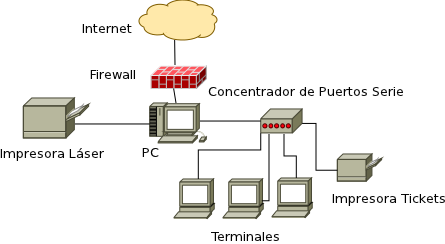
\includegraphics[scale=0.7]{diagrama_ph_sus_1.png}
 \end{center}
 \caption{Sistema en restaurantes}
 \label{fig:sist_rest}
\end{figure}





\end{document}
